\chapter{Receiver calibration}\label{chap:calibration}

% **************************** Define Graphics Path **************************
\ifpdf
    \graphicspath{{calibration/figs/Raster/}{calibration/figs/PDF/}{calibration/figs/}}
\else
    \graphicspath{{calibration/figs/Vector/}{calibration/figs/}}
\fi


With a working instrument capable of taking measurements in the field, the next step towards detection of the 21-cm signature is calibration of the experimental apparatus. There are many forms of calibration from physical antenna or ground plane modifications to numerical post-processing methods such as correctional atmospheric modelling. The need for more accurate cosmic signal measurements against the cacophony of unwanted noise demands finer degrees of calibration through the development of novel methods. At the current technological aim of millikelvin-level calibration, minute differences in an instrument’s electrical properties can skew spectral measurements enough to hamper a cosmological detection. In the previous chapter, we detailed the system architecture designed to minimise these distortions. Here we present a procedure to calibrate out the remaining systematic effects. The task has encompassed decades of research starting in the 1950’s where \citet{bauer_rothe} and \citet{rothe_dahlke} introduced a wave formulation of noise to microwave systems\footnote{\citet{bauer_rothe} presented in English by \citet{penfield}.} before a mathematical prescription to eliminate these noise waves through the derivation of “noise wave parameters” was conceived by \citet{meys} in 1978. This method, which inspires many contemporary radiometric calibration procedures, relies on the relative differences between sequential measurements of known passive devices to divide out small-timescale variability through a method known as “Dicke switching”, named after famed astronomer Robert Dicke. This relative calibration was utilised into the late 2000’s when \citet{edges_limits} placed a lower limit on the duration of the reionisation epoch at $\Delta z < 0.06$.

It was quickly understood that the extraction of further information from 21-cm experimentation required a more powerful calibration method and work commenced to reformulate the noise wave parameters under an “absolute” calibration procedure which offered a more comprehensive derivation by referencing all measurements to an absolute temperature scale as well as expanding compatibility with instruments of increasing bandwidth \citep{rogersCal}. It was this absolute calibration that was used in the 2018 EDGES measurement where the authors quote a 20 mK calibration accuracy \citep{edgesNature, edgesCal}. In response to the controversy surrounding the EDGES experiment, we have strived to improve the methodology and address discrepancies in the procedure through the introduction of a Bayesian calibration framework which we formulate over the following sections.


% =========================================
\section{Calibration formalism}\label{sec:formalism}
The noise necessitating calibration arises during measurements. For a global experiment such as REACH, we measure a sky temperature $\T{sky}(\Omega, \nu, t)$ as a function of the direction $\Omega$, frequency $\nu$ and time $t$ which can be broken down into two primary components: the global 21-cm signal $T_{21}$ and astrophysical foregrounds $\T{f}$
\begin{equation}
    \label{tsky}
    \T{sky}(\Omega, \nu, t) = T_{21}(\nu) + \T{f}(\Omega, \nu, t).
\end{equation}
Sky signals absorbed by the antenna convolve with the normalised antenna directivity $B$ ,introducing systematic noise represented by our random noise term $N_{\mathrm{data}}$.
\begin{equation}\label{bayestsource}
    D(\nu, t) = \int \T{sky}(\Omega, \nu, t) B(\Omega, \nu)\mathrm{d}\Omega + N_{\mathrm{data}}.
\end{equation}
Thus, our 21-cm signature can be formulated as
\begin{equation}\label{signal}
  T_{21} \approx D(\nu, t) - \int\T{f}(\Omega, \nu, t)B(\Omega, \nu)\mathrm{d}\Omega - N_{\mathrm{data}}.
\end{equation}
A diagram illustrating the evolution of the sky signal during this process in shown in \cref{fig:nsfig}.
\begin{figure}
    \centering
    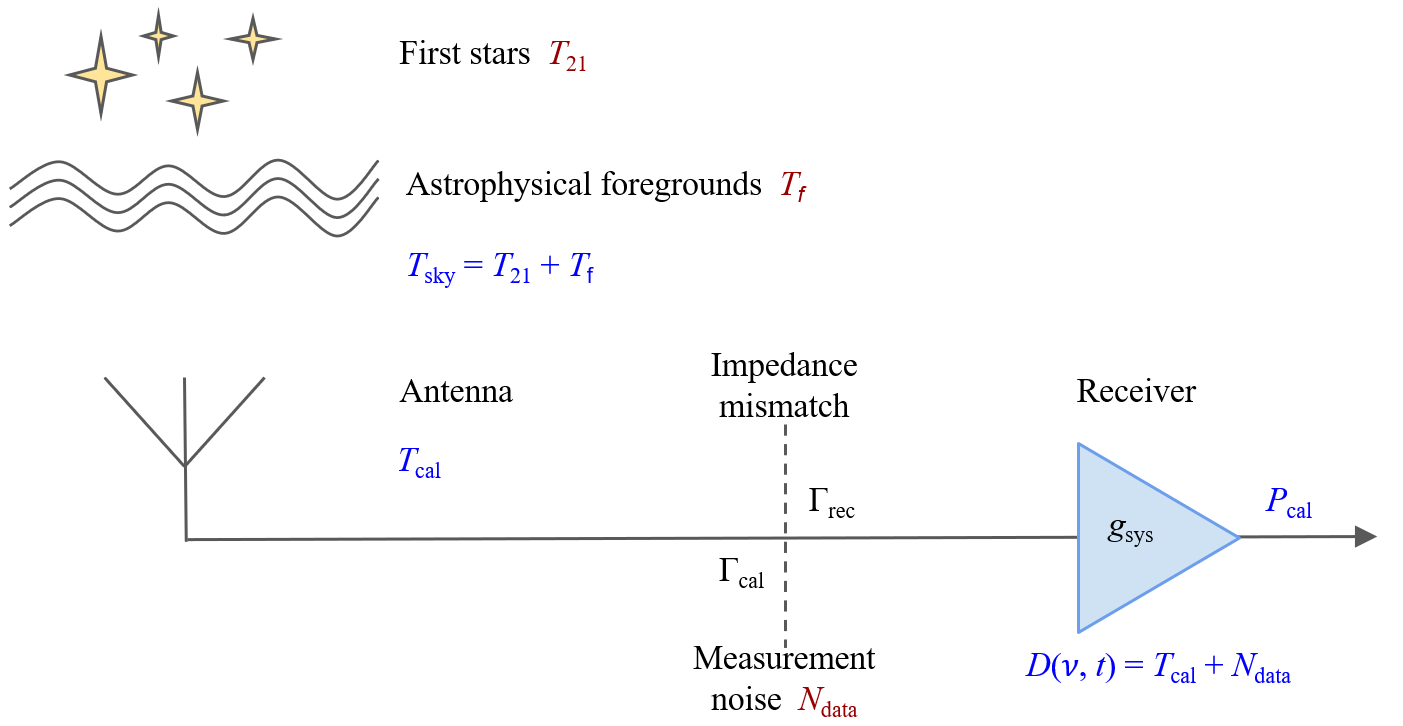
\includegraphics[width=.7\textwidth]{nsdiag}
    \caption{Diagram showing the evolution of the 21-cm signal hampered by astrophysical foregrounds, convolvution with the antenna beam and the emergence of measurement noise before calibration to retrieve the sky temperature.}
    \label{fig:nsfig}
\end{figure}
The integral in \cref{signal} is assessed through foreground and beam modelling techniques such as those discussed in \citet{dom} while modelling of $N_{\mathrm{data}}$ from the (statistical) properties of $D(\nu, t)$ is accomplished through calibration.

The standard calibration strategy follows the method introduced by Dicke to characterise systematic features in radio-frequency instruments \citep{dickeplus} and is widely used in experiments such as EDGES \citep{edgesCal} and LOFAR \citep{lofarCal} to evaluate the spectral index of the sky's diffuse radio background \citep{rogersCal}. The technique involves measurements of two internal reference standards; a load and a noise source, in addition to a series of external calibration sources attached to the receiver input in lieu of the antenna. Historically these include an ambient-temperature ‘cold’ load, a ‘hot’ load heated to $\sim 400$ K, an open-ended cable and a shorted cable as detailed previously in \cref{fig:dicke}.

During a calibration measurement, power spectral densities (PSDs) are taken of each Dicke switch position; the receiver input ($\psd{cal}$), the internal reference load ($\psd{L}$) and the internal reference noise source ($\psd{NS}$) \citep{edgesCal}. These measurements are used to calculate a preliminary `uncalibrated' antenna temperature $\T{cal}^*$
\begin{equation}
  \label{eqn:tantstar}
  \T{cal}^* = \T{NS} \left(\frac{\psd{cal}-\psd{L}}{\psd{NS}-\psd{L}}\right) + \T{L},
\end{equation}
where $\T{L}$ and $\T{NS}$ are assumptions for the noise temperature of the internal reference load and excess noise temperature of the internal noise source above ambient, respectively. This comparison of sequential power measurements serves as the `relative' calibration which removes time-dependent variations in system gain emerging from individual components or technical capabilities of the instrument \citep{edgesCal}. These PSD measurements can be expanded in terms of specific response contributions with the input power spectra being
\begin{multline}
  \label{eqn:pant}
  \psd{cal} = g_{\mathrm{sys}} \Bigg[ \T{cal}\left(1-|\Ga|^2\right)\left|\frac{\sqrt{1 - |\G{rec}|^2}}{1-\Ga\G{rec}}\right|^2 + \T{unc}|\Ga|^2\left|\frac{\sqrt{1 - |\G{rec}|^2}}{1-\Ga\G{rec}}\right|^2 \\
  + \T{cos}\operatorname{Re}\left(\Ga\frac{\sqrt{1 - |\G{rec}|^2}}{1-\Ga\G{rec}}\right) + \T{sin}\operatorname{Im}\left(\Ga\frac{\sqrt{1 - |\G{rec}|^2}}{1-\Ga\G{rec}}\right) 
  + T_0 \Bigg],
\end{multline}
where $\Ga$ and $\G{rec}$ are the measured reflection coefficients of the device connected to the receiver input and receiver itself respectively. $g_{\mathrm{sys}}$ is the system gain referenced to the receiver input and $\T{cal}$ is our calibrated input temperature. $\T{unc}$, $\T{cos}$, and $\T{sin}$ are the ‘noise wave parameters’ introduced by \citet{meys} to calibrate the instrument \footnote{equivalent to $\T{a}$ $\T{b}$, and $\T{c}$ in his notation}. $\T{unc}$ represents the portion of noise reflected by the antenna that is uncorrelated with the output noise of the LNA while $\T{cos}$ and $\T{sin}$ represent the portions correlated with LNA noise \citep{edgesCal, rogersCal}. The phase in which these reflected noise waves re-enter the receiver is described by the Re() and Im() arguments of \cref{eqn:pant}\footnote{These arguments are equivalent to the $\alpha$ term in the EDGES notation \cite{edgesCal} and analogous to $\phi$ in the Meys formulation \citep{meys}}. In the EDGES experiment, the noise wave parameter quantities are modelled using seven-term polynomials in frequency.

The PSDs for the internal reference load and noise source can similarly be expressed as in \cref{eqn:pant}. However, since the reflection coefficients of the internal references are assumed to be small, we approximate them as zeros in order to simplify the equations
\begin{equation}
  \label{eqn:pl}
  \psd{L} = g_{\mathrm{sys}}^*[\T{L}\left(1-|\G{rec}|^2\right)+T_{0}^*],
\end{equation}
\begin{equation}
  \label{eqn:pns}
  \psd{NS} = g_{\mathrm{sys}}^*[\left(\T{L}+\T{NS}\right)\left(1-|\G{rec}|^2\right)+T_{0}^*].
\end{equation}
As shown in \cref{fig:dicke}, the internal references may be on a separate reference plane than the receiver input, resulting in a system gain $g_{\mathrm{sys}}^*$ and a noise offset $T_{0}^*$ different from those defined in \cref{eqn:pant}. This effect is taken into account by two additional scale and offset parameters, $C_1$ and $C_2$, introduced by EDGES \citep{edgesCal}.

Since $C_1$ and $C_2$ also correct for first-order assumptions in the noise temperatures of the internal reference load and noise source, we have chosen to absorb these terms into $\T{L}$ and $\T{NS}$ in our analysis. This adjustment allows all calibration parameters, $\T{unc}$, $\T{cos}$, $\T{sin}$, and the ‘effective’ $\T{NS}$ and $\T{L}$, to be solved for in units of kelvin, facilitating a joint solution of parameters. Expanding \cref{eqn:tantstar} using \cref{eqn:pant,eqn:pl,eqn:pns} yields a linear identity providing a relationship between the uncalibrated input temperature and a final calibrated temperature of any device connected to the receiver input
\begin{multline}
  \label{eqn:caleqn}
  \T{NS}\left( \frac{\psd{cal} - \psd{L}}{\psd{NS} - \psd{L}} \right) + \T{L} = \T{cal}\left[ \frac{1-|\Ga|^2}{|1-\Ga\G{rec}|^2} \right]
  + \T{unc}\left[ \frac{|\Ga|^2}{|1-\Ga\G{rec}|^2} \right] \\
  + \T{cos}\left[ \frac{\operatorname{Re}\left(\frac{\Ga}{1-\Ga\G{rec}}\right)}{\sqrt{1-|\G{rec}|^2}} \right]
  + \T{sin}\left[ \frac{\operatorname{Im}\left(\frac{\Ga}{1-\Ga\G{rec}}\right)}{\sqrt{1-|\G{rec}|^2}} \right],
\end{multline}
where all parameters are frequency-dependent though not explicitly shown for simplicity of notation. During a calibration procedure, $\T{cal}$, $\Ga$ and $\G{rec}$ are measured along with the PSDs while $g_{\mathrm{sys}}$ and $\T{0}$ are calibrated out via the `relative' calibration procedure inherent to \cref{eqn:tantstar}. As stated in \cref{sec:frontend}, the $50 \Omega$ cold and hot loads exhibit the main temperature references needed for $\T{L}$ and $\T{NS}$ while delayed reflection in the calibration cables allow for the derivation of $\T{unc}$, $\T{cos}$ and $\T{sin}$ by simulating an antenna observing an ambient temperature sky \citep{rogersCal}.


% =========================================
\section{Bayesian parameter derivation}\label{sec:bayes}